\section{Performance of Lattice QCD Application}

This section describes the evaluations of XACC performance and productivity for a lattice quantum chromodynamics (Lattice QCD) application.

\subsection{Overview of Lattice QCD}
The Lattice QCD is a discrete formulation of QCD that describes the strong interaction among ``quarks'' and ``gluons.''
While the quark is a species of elementary particles, the gluon is a particle that mediates the strong interaction.
The Lattice QCD is formulated on a four-dimensional lattice (time: T and space:ZYX axes).
We impose a periodic boundary condition in all the directions.
The quark degree of freedom is represented as a field that has four components of ``spin'' and three components of ``color,''
namely a complex vector of $12 \times N_{site}$ components,
where $N_{site}$ is the number of lattice sites.
The gluon is defined as a $3\times 3$ complex matrix field on links (bonds between neighboring lattice sites).
During a Lattice QCD simulation,
one needs to solve many times a linear equation for the matrix that represents the interaction between the quark and gluon fields.
This linear equation is the target of present work.
The matrix acts on the quark vector and has nonzero components only for the neighboring sites, and thus sparse.

\subsection{Implementation}
We implemented a Lattice QCD code based on the existing Lattice QCD application Bridge++\cite{bridge++}.
Since our code was implemented by extracting the main kernel of the Bridge++,
it can be used as a mini-application to investigate its productivity and performance more easily than
use of the original Bridge++.

\begin{figure}[h]
\centering
\begin{minipage}{0.45\hsize}
\begin{lstlisting}
S = B
R = B
X = B
sr = norm(S)
T = WD(U,X)
S = WD(U,T)
R = R - S
P = R
rr = norm(R)
rrp = rr
do{
\end{lstlisting}
\end{minipage} \hspace{0.5cm}
\begin{minipage}{0.45\hsize}
\begin{lstlisting}[firstnumber=10]
  T = WD(U,P)
  V = WD(U,T)
  pap = dot(V,P)
  cr = rr/pap
  X = cr * P + X
  R = -cr * V + R
  rr = norm(R)
  bk = rr/rrp
  P = bk * P + R
  rrp = rr
}while(rr/sr > 1.E-16)
\end{lstlisting}
\end{minipage}
\caption{Lattice QCD pseudo code}\label{fig:pseudo}
\end{figure}

Fig. \ref{fig:pseudo} shows a pseudo code of the implementation,
where the CG method is used to solve quark propagators.
In Fig. \ref{fig:pseudo},
{\it WD()} is the Wilson-Dirac operator\cite{PhysRevD.10.2445},
{\it U} is a gluon, the other uppercase characters are quarks.
The Wilson-Dirac operator is a main kernel in the Lattice QCD,
which calculates how the quarks interact with each other under the influence of the gluon.

\begin{figure}[h]
\centering
\begin{lstlisting}
typedef struct Quark {
 double v[4][3][2];
} Quark_t;
typedef struct Gluon {
 double v[3][3][2];
} Gluon_t;
Quark_t v[NT][NZ][NY][NX], tmp_v[NT][NZ][NY][NX];
Gluon_t u[4][NT][NZ][NY][NX];

#pragma xmp template t[NT][NZ]
#pragma xmp nodes n[NODES_T][NODES_Z]
#pragma xmp distribute t[block][block] onto n
#pragma xmp align v[i][j][*][*] with t[i][j]
#pragma xmp align tmp_v[i][j][*][*] with t[i][j]
#pragma xmp align u[*][i][j][*][*] with t[i][j]
#pragma xmp shadow v[1:1][1:1][0][0]
#pragma xmp shadow tmp_v[1:1][1:1][0][0]
#pragma xmp shadow u[0][1:1][1:1][0][0]
...
int main(){
...
#pragma acc enter data copyin(v, tmp_v, u)
\end{lstlisting}
\caption{Declaration of distributed arrays for Lattice QCD}\label{fig:distributedQCD}
\end{figure}

Fig. \ref{fig:distributedQCD} shows how to declare distributed arrays of the quark and gluon.
In lines 1-8, the quark and gluon structure arrays are declared.
The last dimension ``[2]'' of both structures represents real and imaginary parts for a complex number.
{\it NT}, {\it NZ},  {\it NY} and {\it NX} are the numbers of TZYX axis elements.
In lines 10-18, distributed arrays are declared where the macro constant values {\it NODES\_T} and {\it NODES\_Z} indicate the number of {\tt nodes} on the T and Z axes.
Thus,
the program is parallelized on T and Z axes.
Note that an ``*'' in the {\bf align} directive means that the dimension is not divided.
In the {\bf shadow} directive,
halo regions are added to the arrays because each quark and gluon element is affected by its neighboring orthogonal elements.
Note that ``0'' in the {\bf shadow} directive means that no halo region exists.
In line 22,
the {\bf enter data} directive transfers the distributed arrays from host memory to accelerator memory.

\begin{figure}[h]
\centering
\begin{lstlisting}
#pragma xmp reflect(v) width(/periodic/1:1,/periodic/1:1,0,0) orthogonal acc
#pragma xmp reflect(u) width(0,/periodic/1:0,/periodic/1:0,0,0) orthogonal acc
WD(tmp_v, u, v);
#pragma xmp reflect(tmp_v) width(/periodic/1:1,/periodic/1:1,0,0) orthogonal acc
WD(v, u, tmp_v);
\end{lstlisting}
\caption{Calling Wilson-Dirac operator}\label{fig:callingDirac}
\end{figure}

Fig. \ref{fig:callingDirac} shows how to call {\it WD()}.
The  {\bf reflect} directives are inserted before {\it WD()} in order to update own halo region.
In line 2,
``1:0'' in {\bf width} clause means only the lower halo region is updated because only it is needed in {\it WD()}.
The {\it u} is not updated before the second {\it WD()} function because values of {\it u} are not updated in {\it WD()}.
Moreover,
the {\bf orthogonal} clause is added because diagonal updates of the arrays are not required in {\it WD()}.

\begin{figure}[h]
\centering
\begin{lstlisting}
void WD(Quark_t v_out[NT][NZ][NY][NX], const Gluon_t u[4][NT][NZ][NY][NX], const Quark_t v[NT][NZ][NY][NX])
{
#pragma xmp align v_out[i][j][*][*] with t[i][j]
#pragma xmp align u[*][i][j][*][*] with t[i][j]
#pragma xmp align v[i][j][*][*] with t[i][j]
#pragma xmp shadow v_out[1:1][1:1][0][0]
#pragma xmp shadow u[0][1:1][1:1][0][0]
#pragma xmp shadow v[1:1][1:1][0][0]
 ...
#pragma xmp loop (t,z) on t[t][z]
#pragma acc parallel loop collapse(4) present(v_out, u, v)
 for(int t=0;t<NT;t++)
  for(int z=0;z<NZ;z++)
   for(int y=0;y<NY;y++)
    for(int x=0;x<NX;x++){
\end{lstlisting}
\caption{A portion of Wilson-Dirac operator}\label{fig:dirac}
\end{figure}

Fig. \ref{fig:dirac} shows a part of the Wilson-Dirac operator code.
All arguments in {\it WD()} are distributed arrays.
In XMP and XACC,
distributed arrays which are used as arguments must be redeclared in function to pass their information to a compiler.
Thus, the {\bf align} and {\bf shadow} directives are used in {\it WD()}.
In line 10, the {\bf loop} directive parallelizes the outer two loop statements.
In line 11, the {\bf parallel loop} directive parallelizes all loop statements.
In the loop statements,
a calculation needs neighboring and orthogonal elements.
Note that while the {\it WD()} updates only the {\it v\_out},
it only refers the {\it u} and {\it v}.

\begin{figure}[h]
\centering
\begin{lstlisting}
double norm(const Quark_t v[NT][NZ][NY][NX])
{
#pragma xmp align v[i][j][*][*] with t[i][j]
#pragma xmp shadow v[1:1][1:1][0][0]
 double a = 0.0;

#pragma xmp loop (t,z) on t[t][z]
#pragma acc parallel loop collapse(7) present(v) reduction(+:a)
 for(int t=0;t<NT;t++)
  for(int z=0;z<NZ;z++)
   for(int y=0;y<NY;y++)
    for(int x=0;x<NX;x++)
     for(int i=0;i<4;i++)
      for(int j=0;j<3;j++)
       for(int k=0;k<2;k++)
        a += v[t][z][y][x].v[i][j][k]*v[t][z][y][x].v[i][j][k];

#pragma xmp reduction (+:a)
 return a;
}
\end{lstlisting}
\caption{L2 norm calculation code}\label{fig:norm}
\end{figure}

Fig. \ref{fig:norm} shows L2 norm calculation code in the CG method.
In line 8,
the {\bf reduction} clause performs a reduction operation for the variable {\it a} in each accelerator when finishing the next loop statement.
The calculated variable {\it a} is located in both host memory and accelerator memory.
However, at this point,
all {\tt nodes} have individual values of {\it a}.
To obtain the total value of the variable {\it a},
the XMP {\bf reduction} directive in line 18 also performs a reduction operation among {\tt nodes}.
Since the total value is used on only host after this function,
the XMP {\bf reduction} directive does not have {\bf acc} clause.

\section{Performance Evaluation}\label{sec:performance}
\subsection{Result}
\begin{table}[h]
\renewcommand{\arraystretch}{1.2}
\centering
\caption{Evaluation environment} \label{tab:ha-pacs/tca}
\begin{tabular}{l|l}\hline
CPU & Intel Xeon-E5 2680v2 2.8 GHz x 2 Sockets \\
Memory & DDR3 1866MHz 59.7GB/s 128GB \\
GPU & NVIDIA Tesla K20X (GDDR5 250GB/s 6GB) x 4 GPUs \\
Network & InfiniBand Mellanox Connect-X3 Dual-port QDR 8GB/s \\
\multirow{2}{*}{Software} & Intel 16.0.2, CUDA 7.5.18, Omni OpenACC compiler 1.1\\
 & MVAPICH2 2.1\\ \hline
\end{tabular}
\end{table}

This section evaluates the performance level of XACC on the Lattice QCD code.
For comparison purposes,
those of MPI+CUDA and MPI+OpenACC are also evaluated.
For performance evaluation,
we use the HA-PACS/TCA system\cite{hapacs} the hardware specifications and software environments of which are shown in Table \ref{tab:ha-pacs/tca}.
Since each compute node has four GPUs,
we assign four {\tt nodes} per compute node and direct each {\tt node} to deal with a single GPU.
We use the Omni OpenACC compiler\cite{2013tabuchi} as a backend compiler in the Omni XACC compiler.
We execute the Lattice QCD codes with strong scaling in regions (32,32,32,32) as ({\it NT},{\it NZ},{\it NY},{\it NX}).
The Omni XACC compiler provides various types of data communication among accelerators\cite{nakao2014}.
We use the MPI+CUDA implementation type because it provides a balance of versatility and performance.

\begin{figure}[h]
\centering
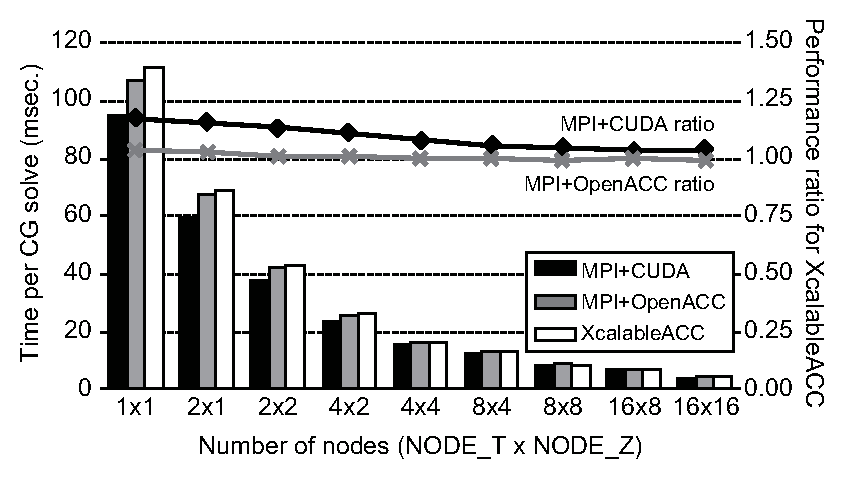
\includegraphics[scale=0.58,clip]{figs/performance32.eps}
\caption{Performance results} \label{fig:performance}
\end{figure}

Fig. \ref{fig:performance} shows the performance results that indicate the time required to solve one CG iteration as well as the performance ratio values that indicate the comparative performance \
of XACC and other languages.
When the performance ratio value of a language is greater than 1.00,
the performance result of the language is better than that of XACC.
Fig. \ref{fig:performance} shows that the performance ratio values of MPI+CUDA are between 1.04 and 1.18,
and that those of MPI+OpenACC are between 0.99 and 1.04.
Moreover,
Fig. \ref{fig:performance} also shows that the performance results of both MPI+CUDA and MPI+OpenACC become closer to those of XACC as the number of {\tt nodes} increases.

\subsection{Discussion}
To examine the performance levels in detail,
we measure the time required for the halo updating operation for two {\tt nodes} and more.
The halo updating operation consists of the communication and pack/unpack processes for non-contiguous regions in the XACC runtime.

\begin{figure}[h]
\centering
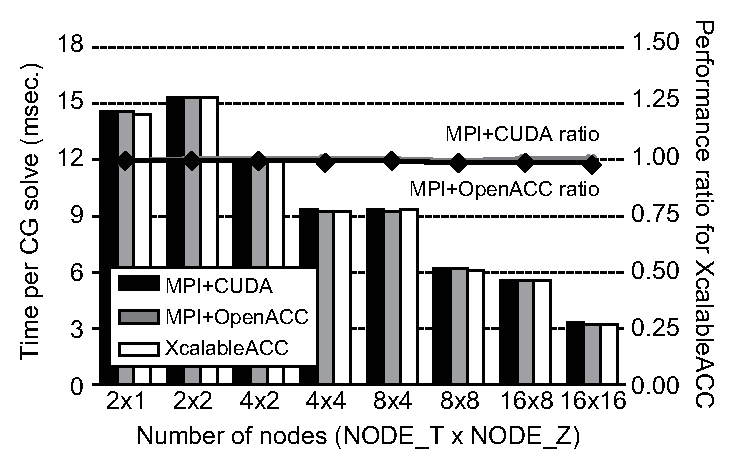
\includegraphics[scale=0.58,clip]{figs/halo-comm.eps}
\caption{Communication time} \label{fig:halo-comm}
\end{figure}

\begin{figure}[h]
\centering
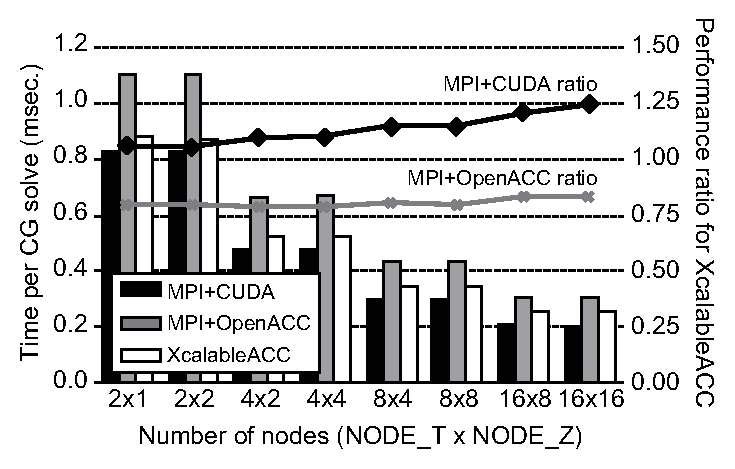
\includegraphics[scale=0.58,clip]{figs/halo-pack-unpack.eps}
\caption{Pack/unpack time} \label{fig:halo-pack-unpack}
\end{figure}

While Fig. \ref{fig:halo-comm} describes communication time of the halo updating time of Fig \ref{fig:performance},
Fig. \ref{fig:halo-pack-unpack} describes pack/unpack time of it.
Fig. \ref{fig:halo-comm} shows that
the communication performance levels of all implementations are almost the same.
However,
Fig. \ref{fig:halo-pack-unpack} shows that the pack/unpack performance levels of MPI+CUDA are better than those of XACC,
and that those of MPI+OpenACC are worse than those of XACC.
The reason for the pack/unpack operation performance level difference is that the XACC operation is implemented in CUDA at XACC runtime.
Thus,
some performance levels of XACC are better than those of MPI+OpenACC in Fig. \ref{fig:performance}.
However,
the performance levels of XACC in Fig. \ref{fig:halo-pack-unpack} is worse than those of MPI+CUDA because XACC requires the cost of XACC runtime calls.

\begin{figure}[h]
\centering
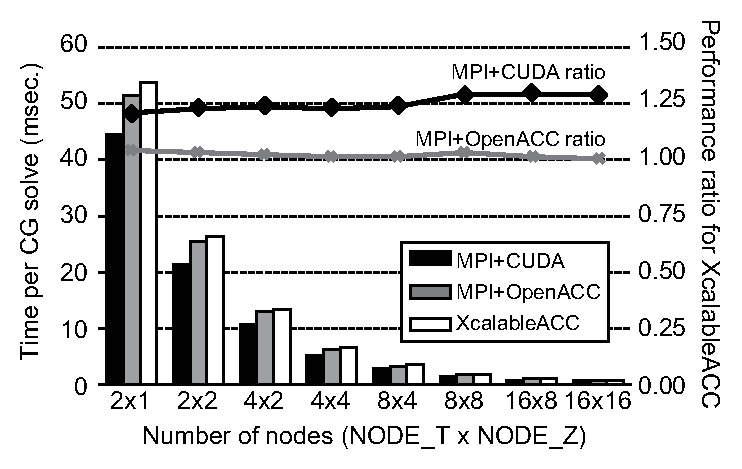
\includegraphics[scale=0.58,clip]{figs/exceptforhalo.eps}
\caption{Time excluding halo updating time} \label{fig:exceptforhalo}
\end{figure}

Fig. \ref{fig:exceptforhalo} shows the overall time excluding the halo updating time,
where performance levels of MPI+CUDA are the best, and those of XACC are almost the same as those of MPI+OpenACC.
The reason for the difference is due to how to use GPU threads.
In the CUDA implementation,
we assign loop iterations to GPU threads in a cyclic-manner manually.
In contrast, in the OpenACC and XACC implementations,
how to assign GPU threads is an implementation dependent of an OpenACC compiler.
In the Omni OpenACC compiler,
initially loop iterations are assigned to GPU threads by a gang (threadblock) in a block manner,
and then are also assigned to them by a vector (thread) in a cyclic manner.
With the {\bf gang} clause with the {\bf static} argument proposed in the OpenACC specification version 2.0,
programmers can determine how to use GPU threads to some extent,
but the Omni OpenACC compiler does not yet support it.

\begin{figure}[h]
\centering
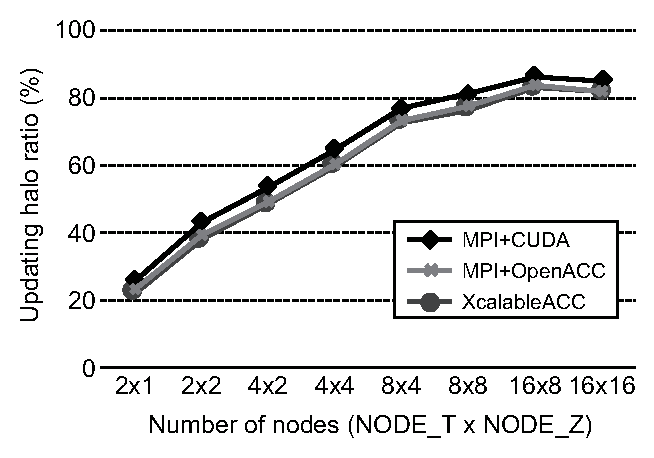
\includegraphics[scale=0.58,clip]{figs/exceptforhalo-per.eps}
\caption{Updating halo ratio} \label{fig:exceptforhalo-per}
\end{figure}

Fig. \ref{fig:exceptforhalo-per} shows the ratio of the halo updating time to overall time.
As can be seen,
as the number of {\tt nodes} increases, the ratio increases as well.
Therefore,
when a large number of {\tt nodes} are used,
there is little difference in performance level of Fig. \ref{fig:performance} among the three implementations.
The reason why the ratio of MPI+CUDA is slightly larger than those of the others is that
the time excluding the halo communication of MPI+CUDA in Fig. \ref{fig:halo-comm} is relatively small.

\section{Productivity Improvement}
\subsection{Requirement for Productive Parallel Language}
\begin{figure}[h]
\centering
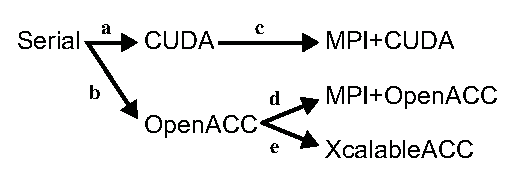
\includegraphics[scale=0.75,clip]{figs/howtocreate1.eps}
\caption{Application development order on accelerated cluster} \label{fig:howtocreate}
\end{figure}

In Section \ref{sec:performance},
we developed three Lattice QCD codes using MPI+CUDA, MPI+OpenACC, and XACC.
Fig. \ref{fig:howtocreate} shows our procedure for developing each code where
we first develop the code for an accelerator from the serial code,
and then extend it to handle an accelerated cluster.

To parallelize the serial code for an accelerator using CUDA requires large code changes (``a'' in Fig. \ref{fig:howtocreate}),
most of which are necessary to create new kernel functions and to make 1D arrays out of multi-dimensional arrays.
By contrast,
OpenACC accomplishes the same parallelization with just small code changes (``b''),
because OpenACC's directive-based approach encourages reuse of an existing code.
Besides,
to parallelize the code for a distributed memory system,
MPI also requires large changes (``c'' and ``d''),
primarily to convert global indices into local indices.
By contrast,
XACC requires smaller code changes (``e'') because XACC is also directive-based language as OpenACC.

In many cases,
a parallel code for an accelerated cluster is based on an existing serial code.
The code changes to the existing serial code are likely to trigger program bugs.
Therefore,
XACC is designed to reuse an existing code as possible.

\subsection{Quantitative Evaluation by Delta Source Lines of Codes}
\begin{table}[h]
\renewcommand{\arraystretch}{1.2}
\centering
\caption{DSLOC of Lattice QCD implementations} \label{tab:dsloc}
\begin{tabular}[h]{r|rrrrr|rrr} \hline
       & a   & b  & c   & d   & e   & a+c & b+d & {\bf b+e}  \\ \hline
DSLOC  & 552 & 22 & 280 & 201 & 138 & 832 & 223 & {\bf 160} \\  \hline
Add    & 137 & 20 & 185 & 140 & 134 & 322 & 160 & {\bf 154} \\
Delete & 73 & 0 & 0 & 0 & 0 & 73 & 0 & {\bf 0} \\
Modify & 342 & 2 & 95 & 61 & 4 & 437 & 63 & {\bf 6} \\ \hline
\end{tabular}
\end{table}

As one of metrics for productivity,
Delta Source Lines of Codes (DSLOC) is proposed\cite{CGPOP2011}.
The DSLOC indicates how the codes change from a corresponding implementation.
The DSLOC is the sum of three components: how many lines are added, deleted and modified.
When the DSLOC is small,
the programming costs and the possibility of program bugs will be small as well.
We use the DSLOC to count the amount of change required to implement an accelerated cluster code from a serial code.

Table \ref{tab:dsloc} shows the DSLOC where lowercase characters correspond to Fig. \ref{fig:howtocreate}.
The DSLOC of XACC (b+e) is smaller than MPI+CUDA (a+c) and MPI+OpenACC (b+d).
The difference between XACC and MPI+CUDA is 420.0\%, and that between XACC and MPI+OpenACC is 39.4\%.

\subsection{Discussion}\label{sec:pro-con}
\begin{figure}[h]
\centering
\begin{lstlisting}
#pragma acc parallel loop collapse(4) present(v_out, u, v)
 for(int t=0;t<NT;t++)
  for(int z=0;z<NZ;z++)
   for(int y=0;y<NY;y++)
    for(int x=0;x<NX;x++){
     int tt = (t + 1) % NT;
     v_out[tt][z][y][x].v[0][0][0] = ... ;
\end{lstlisting}\vspace{-1.5ex}
\caption{Code modification of {\it WD()} in OpenACC}\label{fig:modification-openacc}
\end{figure}

\begin{figure}[h]
\centering
\begin{lstlisting}
#pragma xmp loop (t,z) on t[t][z]
#pragma acc parallel loop collapse(4) present(v_out, u, v)
 for(int t=0;t<NT;t++)
  for(int z=0;z<NZ;z++)
   for(int y=0;y<NY;y++)
    for(int x=0;x<NX;x++){
     int tt = t + 1;
     v_out[tt][z][y][x].v[0][0][0] = ... ;
\end{lstlisting}\vspace{-1.5ex}
\caption{Code modification of {\it WD()} in XcalableACC}\label{fig:modification-xacc}
%\caption{Code modification in {\it WD()}} \label{fig:modification}
\end{figure}

In ``e'' of Table \ref{tab:dsloc},
four lines for modification are required to implement the XACC code from the OpenACC code.
Fig. \ref{fig:modification-openacc} and \ref{fig:modification-xacc} show the modification,
which is a part of {\it WD()} of Fig. \ref{fig:dirac}.
A variable {\it tt} is used to be an index for halo region.
The {\it tt} is modified from line 6 of Fig. \ref{fig:modification-openacc} to line 7 of Fig. \ref{fig:modification-xacc}.
In Fig. \ref{fig:modification-openacc},
when a value of a variable {\it t} is ``{\it NT}-1'',
that of the variable {\it tt} becomes ``0'' which is the lower bound index of the first dimension of the array {\it v\_out}.
On the other hand,
in Fig. \ref{fig:modification-xacc},
communication of the halo is performed before execution of {\it WD()} by the {\bf reflect} directive shown in Fig. \ref{fig:callingDirac}.
Thus,
the variable {\it tt} need only be incremented in Fig. \ref{fig:modification-xacc}.
There are four such modifications in {\it WD()}.
Note that
XACC does not keep the semantics of the base code perfectly in this case
in exchange for simplified parallelization.
In addition,
there are two lines for modification shown in ``b'' of Table \ref{tab:dsloc}.
It is a very fine modification for OpenACC constraints,
which keeps the semantics of the base code.

\begin{table}[h]
\renewcommand{\arraystretch}{1.2}
\centering
\caption{SLOC of Lattice QCD implementations} \label{tab:sloc}
\begin{tabular}[h]{r|rrr} \hline
               & MPI+CUDA & MPI+OpenACC & {\bf XcalableACC}  \\ \hline
SLOC           & 1091     & 1002        & {\bf 996} \\ \hline
\#XcalableMP   & -        & -           & {\bf 122} \\
\#OpenACC      & -        & 26          & {\bf 16}  \\
\#XcalableACC  & -        & -           & {\bf 3}   \\
\#MPI function & 39       & 39          & {\bf -}   \\ \hline
\end{tabular}
\end{table}

\begin{figure}[h]
\centering
\begin{lstlisting}
void WD(Quark_t v_out[NT][NZ][NY][NX], const Gluon_t u[4][NT][NZ][NY][NX], const Quark_t v[NT][NZ][NY][NX])
{
#pragma xmp align [i][j][*][*] with t[i][j] shadow [1:1][1:1][0][0] :: v_out, v
#pragma xmp align [*][i][j][*][*] with t[i][j] shadow [0][1:1][1:1][0][0] :: u
\end{lstlisting}
\caption{New directive combination syntax that applies to Fig. \ref{fig:dirac}}\label{fig:combine}
\end{figure}

As basic information,
we count the source lines of codes (SLOC) of each of the Lattice QCD implementations.
Table \ref{tab:sloc} shows the SLOC excluding comments and blank lines,
as well as the numbers of each directive and MPI functions included in their SLOC.
For reader information,
SLOC of the serial version Lattice QCD code is 842.
Table \ref{tab:sloc} shows that
the 122 XMP directives are used in the XACC implementation,
many of which are declarations for function arguments.
To reduce the XMP directives,
we are planning to develop a new syntax that combines declarations with the same attribute into one directive.
Fig. \ref{fig:combine} shows an example of the new syntax applied to the declarations in Fig. \ref{fig:dirac}.
Since the arrays {\it v\_out} and {\it v} have the same attribute,
they can be declared into a single XMP directive.
Moreover,
the {\bf shadow} directive attribute is added to the {\bf align} directive as its clause.
When applying the new directive to XACC implementation,
the number of XMP directives decreases from the 122 shown in Table \ref{tab:sloc} to 64,
and the XACC DSLOC decreases from the 160 shown in Table \ref{tab:dsloc} to 102.
